\documentclass[a4paper,12pt]{article}
\usepackage[utf8]{inputenc}
\usepackage[english]{babel}
\usepackage{graphicx}
\usepackage{geometry}
\usepackage{listings}
\usepackage{xcolor}
\usepackage{tikz}
\usetikzlibrary{shapes, arrows, positioning}

\geometry{top=2cm, bottom=2cm, left=2.5cm, right=2.5cm}

% Code snippet style setup (same as your previous file)
\definecolor{codegreen}{rgb}{0,0.6,0}
\lstdefinestyle{mystyle}{
    backgroundcolor=\color{white},   
    commentstyle=\color{codegreen},
    keywordstyle=\color{blue},
    basicstyle=\ttfamily\footnotesize,
    breakatwhitespace=false,         
    breaklines=true,                 
    captionpos=b,                    
    keepspaces=true,              
    numbers=left,                    
    numbersep=5pt,                  
    showspaces=false,                
    showstringspaces=false,
    showtabs=false,                  
    tabsize=2,
    frame=single
}
\lstset{style=mystyle}

\title{\textbf{Practical Work 3: File Transfer using MPI}}
\author{Group ID: 16}
\date{\today}

\begin{document}

\maketitle

\section{Introduction}
The objective of this practical work is to upgrade a standard TCP file transfer system into a distributed system using the \textbf{Message Passing Interface (MPI)} standard. The goal is to transfer a file from a Sender process to a Receiver process within an MPI environment.

\section{MPI Implementation Choice}
We chose \textbf{Python} with the \textbf{mpi4py} library for this implementation. 
\begin{itemize}
    \item \textbf{Reasoning:} Python offers high-level readability, and \texttt{mpi4py} provides Pythonic bindings for the standard MPI standard (like OpenMPI or MPICH). It allows passing arbitrary Python objects (picklable) as well as efficient direct memory buffers (byte-like objects), making it ideal for prototyping file transfer logic.
\end{itemize}

\section{System Design}

\subsection{Architecture}
The system follows a \textbf{Master-Slave} (or Peer-to-Peer) pattern where:
\begin{itemize}
    \item \textbf{Rank 0 (Sender):} Reads the file from the disk and transmits metadata (name, size) followed by data chunks.
    \item \textbf{Rank 1 (Receiver):} Listens for metadata, creates a destination file, and writes the incoming data chunks until an End-of-File (EOF) signal is received.
\end{itemize}

\subsection{Data Flow Diagram}
The figure below illustrates the communication protocol between the MPI ranks:

\begin{figure}[h]
    \centering
    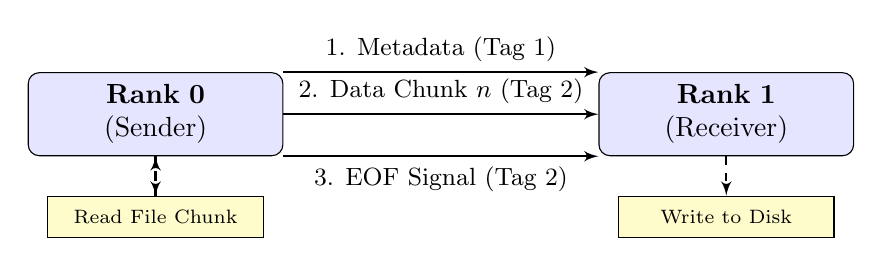
\begin{tikzpicture}[
        node distance=2cm and 3cm,
        block/.style={rectangle, draw, fill=blue!10, text width=3cm, text centered, rounded corners, minimum height=3em},
        data/.style={rectangle, draw, fill=yellow!20, text width=2.5cm, text centered, minimum height=1.5em, font=\scriptsize},
        line/.style={draw, -latex', thick}
    ]
    % Nodes
    \node [block] (sender) {\textbf{Rank 0} \\ (Sender)};
    \node [block, right=4cm of sender] (receiver) {\textbf{Rank 1} \\ (Receiver)};
    
    % Data Flows
    \path [line] (sender.north east) -- node[above, font=\small] {1. Metadata (Tag 1)} (receiver.north west);
    \path [line] (sender.east) -- node[above, font=\small] {2. Data Chunk $n$ (Tag 2)} (receiver.west);
    \path [line] (sender.south east) -- node[below, font=\small] {3. EOF Signal (Tag 2)} (receiver.south west);
    
    % Internal actions
    \node [data, below=0.5cm of sender] (read) {Read File Chunk};
    \node [data, below=0.5cm of receiver] (write) {Write to Disk};
    
    \path [line, dashed] (sender) -- (read);
    \path [line, dashed] (read) -- (sender);
    \path [line, dashed] (receiver) -- (write);
    
    \end{tikzpicture}
    \caption{MPI File Transfer Communication Flow}
    \label{fig:mpi_flow}
\end{figure}

\section{Implementation}

\subsection{Sender Logic (Rank 0)}
The sender handles file I/O and non-blocking transmission logic.
\begin{lstlisting}[language=Python, caption=Sender Function]
def sender(self):
    # Send metadata
    self.comm.send({'name': self.filename, 'size': size}, dest=1, tag=1)
    
    # Send content loop
    with open(self.filename, 'rb') as f:
        while True:
            chunk = f.read(self.chunk_size)
            if not chunk: break
            self.comm.send(chunk, dest=1, tag=2)
            
    # Send termination signal
    self.comm.send(None, dest=1, tag=2)
\end{lstlisting}

\subsection{Receiver Logic (Rank 1)}
The receiver waits for specific tags to reconstruct the file.
\begin{lstlisting}[language=Python, caption=Receiver Function]
def receiver(self):
    # Receive metadata
    meta = self.comm.recv(source=0, tag=1)
    new_name = "received_" + meta['name']
    
    # Receive loop
    with open(new_name, 'wb') as f:
        while True:
            chunk = self.comm.recv(source=0, tag=2)
            if chunk is None: break
            f.write(chunk)
\end{lstlisting}

\section{Roles and Responsibilities}
\begin{table}[h]
\centering
\begin{tabular}{|c|l|l|}
\hline
\textbf{No.} & \textbf{Member} & \textbf{Task} \\ \hline
1 & Member 1 & MPI Environment Setup, Sender Logic \\ \hline
2 & Member 2 & Receiver Logic, File I/O Handling \\ \hline
3 & Member 3 & Report writing, Architecture diagrams \\ \hline
\end{tabular}
\caption{Group Roles}
\end{table}

\end{document}